%%%%%%%   KRIPKE STRUCTURES
\showCILC{true}{
	\begin{frame}{Description}
		\vspace{2mm}
		\showCILC{true}{
			\onslide<+->{
			\begin{block}{Pointed Kripke structure}
			A \emph{Pointed Kripke structure} is a pair (\tuple{S, \pi, \brelSlide{1},$\dots$ , \brelSlide{n}}, $s_0$), s.t.:
			\begin{itemize}
				\item[-] $S$ is a set of \emphSlide{worlds} and  $s_0 \in S$
				\item[-] $\func{\pi}{S}{2^{\sF}}$ associates an \emphSlide{interpretation} to each element of S
				\item[-] for $1 \leq \defemph{i} \leq \defemph{n}$, $\brelSlide{i} \subseteq S \times S$  is a binary relation over S
			\end{itemize}
		\end{block}
		}
	}
		\begin{columns}
			\onslide<+->{\begin{column}{0.5\textwidth}

					\vspace*{-0.1cm}\hspace*{-0.6cm}\scalebox{0.7} {

\tikzset{every picture/.style={line width=0.75pt}} %set default line width to 0.75pt        

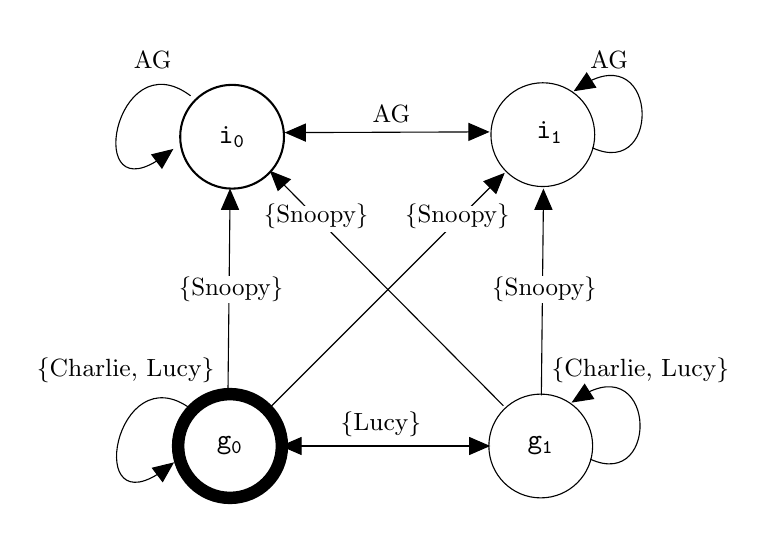
\begin{tikzpicture}[x=0.75pt,y=0.75pt,yscale=-1,xscale=1]
%uncomment if require: \path (0,300); %set diagram left start at 0, and has height of 300

%Curve Lines [id:da6922101751426857] 
\draw    (326.43,51.72) .. controls (366.43,21.72) and (369.63,95.32) .. (334.83,79.32) ;


%Curve Lines [id:da6315070066186073] 
\draw    (141.29,54.27) .. controls (104.49,26.67) and (88.76,113.08) .. (128.76,83.08) ;


%Straight Lines [id:da0043984547546391806] 
\draw    (191.92,72) -- (280.03,71.67) ;


%Straight Lines [id:da8170776057111964] 
\draw    (311.29,104.28) -- (310.29,198.64) ;


%Straight Lines [id:da10125059076875131] 
\draw    (288.88,95.12) -- (177.9,206.1) ;


%Straight Lines [id:da13591440442801073] 
\draw    (183.13,94.02) -- (292,203.6) ;


%Curve Lines [id:da0862450190271058] 
\draw    (141.62,205.27) .. controls (104.82,177.67) and (89.1,264.08) .. (129.1,234.08) ;


%Straight Lines [id:da17405321396390305] 
\draw    (160.29,104.28) -- (159.29,198.64) ;


%Straight Lines [id:da018251469869151382] 
\draw    (185.29,223) -- (285,223) ;

%Curve Lines [id:da8507870813478686] 
\draw    (325.43,201.72) .. controls (365.43,171.72) and (368.63,245.32) .. (333.83,229.32) ;

%Shape: Circle [id:dp9462184779936802] 
\draw   (286,73) .. controls (286,59.19) and (297.19,48) .. (311,48) .. controls (324.81,48) and (336,59.19) .. (336,73) .. controls (336,86.81) and (324.81,98) .. (311,98) .. controls (297.19,98) and (286,86.81) .. (286,73) -- cycle ;
%Shape: Circle [id:dp6359205424734804] 
\draw  [line width=4.5]  (135.29,223) .. controls (135.29,209.19) and (146.48,198) .. (160.29,198) .. controls (174.09,198) and (185.29,209.19) .. (185.29,223) .. controls (185.29,236.81) and (174.09,248) .. (160.29,248) .. controls (146.48,248) and (135.29,236.81) .. (135.29,223) -- cycle ;
%Shape: Circle [id:dp06782137726568571] 
%Shape: Circle [id:dp8938158972072578] 
\draw  [line width=0.75]  (135.29,223) .. controls (135.29,209.19) and (146.48,198) .. (160.29,198) .. controls (174.09,198) and (185.29,209.19) .. (185.29,223) .. controls (185.29,236.81) and (174.09,248) .. (160.29,248) .. controls (146.48,248) and (135.29,236.81) .. (135.29,223) -- cycle ;
%Shape: Circle [id:dp19780391712041556] 
\draw   (285,223) .. controls (285,209.19) and (296.19,198) .. (310,198) .. controls (323.81,198) and (335,209.19) .. (335,223) .. controls (335,236.81) and (323.81,248) .. (310,248) .. controls (296.19,248) and (285,236.81) .. (285,223) -- cycle ;
%Shape: Triangle [id:dp4725710951486233] 
\draw  [fill={rgb, 255:red, 0; green, 0; blue, 0 }  ,fill opacity=1 ] (132.8,231.28) -- (127.82,240.08) -- (122.97,233.67) -- cycle ;
%Shape: Triangle [id:dp08394946096129607] 
\draw  [fill={rgb, 255:red, 0; green, 0; blue, 0 }  ,fill opacity=1 ] (285,223) -- (275.72,227.02) -- (275.72,218.98) -- cycle ;
%Shape: Triangle [id:dp12888926826248426] 
\draw  [fill={rgb, 255:red, 0; green, 0; blue, 0 }  ,fill opacity=1 ] (185.29,223) -- (194.56,218.98) -- (194.56,227.02) -- cycle ;
%Shape: Triangle [id:dp7536519811814515] 
\draw  [fill={rgb, 255:red, 0; green, 0; blue, 0 }  ,fill opacity=1 ] (325.43,201.72) -- (331.13,193.37) -- (335.42,200.17) -- cycle ;


\draw  [line width=0.75]  (136.29,74) .. controls (136.29,60.19) and (147.48,49) .. (161.29,49) .. controls (175.09,49) and (186.29,60.19) .. (186.29,74) .. controls (186.29,87.81) and (175.09,99) .. (161.29,99) .. controls (147.48,99) and (136.29,87.81) .. (136.29,74) -- cycle ;
%Shape: Triangle [id:dp8413979641210945] 
\draw  [fill={rgb, 255:red, 0; green, 0; blue, 0 }  ,fill opacity=1 ] (132.46,80.28) -- (127.49,89.08) -- (122.64,82.67) -- cycle ;
%Shape: Triangle [id:dp417855807516911] 
\draw  [fill={rgb, 255:red, 0; green, 0; blue, 0 }  ,fill opacity=1 ] (160.29,99.64) -- (164.3,108.92) -- (156.27,108.92) -- cycle ;
%Shape: Triangle [id:dp4971926593318259] 
\draw  [fill={rgb, 255:red, 0; green, 0; blue, 0 }  ,fill opacity=1 ] (292.17,91.86) -- (288.41,101.24) -- (282.75,95.53) -- cycle ;

%Shape: Triangle [id:dp5745677700051097] 
\draw  [fill={rgb, 255:red, 0; green, 0; blue, 0 }  ,fill opacity=1 ] (326.43,51.72) -- (332.13,43.37) -- (336.42,50.17) -- cycle ;

%Shape: Triangle [id:dp7023350686012408] 
\draw  [fill={rgb, 255:red, 0; green, 0; blue, 0 }  ,fill opacity=1 ] (284.67,71.67) -- (275.39,75.69) -- (275.39,67.65) -- cycle ;
%Shape: Triangle [id:dp6039108674849356] 
\draw  [fill={rgb, 255:red, 0; green, 0; blue, 0 }  ,fill opacity=1 ] (187.29,72) -- (196.56,67.98) -- (196.56,76.02) -- cycle ;
%Shape: Triangle [id:dp9176823524690971] 
\draw  [fill={rgb, 255:red, 0; green, 0; blue, 0 }  ,fill opacity=1 ] (179.93,90.84) -- (189.24,94.56) -- (183.44,99.82) -- cycle ;
%Shape: Rectangle [id:dp7039913742222839] 
\draw  [color={rgb, 255:red, 0; green, 0; blue, 0 }  ,draw opacity=0 ][fill={rgb, 255:red, 255; green, 255; blue, 255 }  ,fill opacity=1 ] (148.29,141.18) -- (173.29,141.18) -- (173.29,153.97) -- (148.29,153.97) -- cycle ;
%Shape: Triangle [id:dp2216172811102144] 
\draw  [fill={rgb, 255:red, 0; green, 0; blue, 0 }  ,fill opacity=1 ] (311.29,99.64) -- (315.3,108.92) -- (307.27,108.92) -- cycle ;
%Shape: Rectangle [id:dp8761718319086598] 
\draw  [color={rgb, 255:red, 0; green, 0; blue, 0 }  ,draw opacity=0 ][fill={rgb, 255:red, 255; green, 255; blue, 255 }  ,fill opacity=1 ] (299.29,141.18) -- (324.29,141.18) -- (324.29,153.97) -- (299.29,153.97) -- cycle ;
%Shape: Rectangle [id:dp30238976789343086] 
\draw  [color={rgb, 255:red, 0; green, 0; blue, 0 }  ,draw opacity=0 ][fill={rgb, 255:red, 255; green, 255; blue, 255 }  ,fill opacity=1 ] (257.29,107.18) -- (282.29,107.18) -- (282.29,119.97) -- (257.29,119.97) -- cycle ;
%Shape: Rectangle [id:dp8647257034518798] 
\draw  [color={rgb, 255:red, 0; green, 0; blue, 0 }  ,draw opacity=0 ][fill={rgb, 255:red, 255; green, 255; blue, 255 }  ,fill opacity=1 ] (189.29,107.18) -- (214.29,107.18) -- (214.29,119.97) -- (189.29,119.97) -- cycle ;

% Text Node
\draw (160.29,223) node  [align=left] {$\mathtt{g_0}$};
% Text Node
\draw (310,223) node  [align=left] {$\mathtt{g_1}$};
% Text Node
\draw (161.29,74) node  [align=left] {$\mathtt{i_0}$};
% Text Node
\draw (314.29,72) node  [align=left] {$\mathtt{i_1}$};
% Text Node
\draw (238,63) node [scale=0.9] [align=left] {\agentSlide{AG}};
% Text Node
\draw (123,37) node [scale=0.9] [align=left] {\agentSlide{AG}};
% Text Node
\draw (343,37) node [scale=0.9] [align=left] {\agentSlide{AG}};
% Text Node
\draw (160.79,147.58) node [scale=0.9] [align=left] {\{\agentSlide{Snoopy}\}};
% Text Node
\draw (311.79,147.58) node [scale=0.9] [align=left] {\{\agentSlide{Snoopy}\}};
% Text Node
\draw (269.79,112.18) node [scale=0.9] [align=left] {\{\agentSlide{Snoopy}\}};
% Text Node
\draw (201.79,112.18) node [scale=0.9] [align=left] {\{\agentSlide{Snoopy}\}};
% Text Node
\draw (110,186.6) node  [align=left] {{\small \{\agentSlide{Charlie}, \agentSlide{Lucy}\}}};
% Text Node
\draw (358,186.6) node  [align=left] {{\small \{\agentSlide{Charlie}, \agentSlide{Lucy}\}}};
% Text Node
\draw (233,212.6) node  [align=left] {{\small \{\agentSlide{Lucy}\}}};
% Text Node
%\draw (230,33.07) node [scale=0.9] [align=left] {\agentSlide{AG} = \{\agentSlide{Charlie}, \agentSlide{Lucy}, \agentSlide{Snoopy}\}};


\end{tikzpicture}}

				\end{column}
				\begin{column}{0.5\textwidth}

					{\small \vspace*{-1cm}\agentSlide{AG} = \{\agentSlide{Charlie}, \agentSlide{Lucy}, \agentSlide{Snoopy}\}}

					\hspace*{-0.5cm}\includegraphics[width=1\textwidth]{img/goal_state}
				\end{column}}
		\end{columns}

	\end{frame}
}

\showCILC{true}{
	\begin{frame}{Entailment}
		Let $\varphi$ be a belief formula and \state{}{s} be a pointed Kripke structure:
		\begin{block}{Entailment w.r.t. a pointed Kripke structure}
			\begin{itemize}[<+->]
				\item[-] $\state{}{s} \models \varphi$ if $\varphi$ is a \emphSlide{fluent formula} and $\pi(\defemph{s})
					      \models \varphi$;
				\item[-] $\state{}{s} \models \mathbf{B}_{\agentSlide{ag_i}}\varphi$ if $\forall $ \defemph{t}:
				      $\defemph{(s,t)} \in \brelSlide{i}$ it holds that\ $ \state{}{t} \models \varphi$;
				      %\item $\state{}{s} \models \neg \varphi$ if $\state{}{s} \not\models \varphi$;
				      %\item $\state{}{s} \models \varphi_1 \vee \varphi_2$ if $\state{}{s}\models
				      %\varphi_1$ or $\state{}{s}\models \varphi_2$;
				      %\item $\state{}{s} \models \varphi_1 \wedge \varphi_2$ if $\state{}{s}\models
				      %\varphi_1$ and $\state{}{s}\models \varphi_2$;
				\item[-] $\state{}{s} \models \eAlpha{\varphi}$ if $\state{}{s} \models
					      \mathbf{B}_{\agentSlide{ag_i}}{\varphi}$ for all \agentSlide{ag_i} $\in \alpha$;
				\item<.->[-] $\state{}{s} \models \cAlpha{\varphi}$ if
				      $\state{}{s} \models \eAlphaIter{k}{\varphi}$ for every
				      $k\geq0$, where $\eAlphaIter{0}{\varphi} = \varphi$ and
				      $\eAlphaIter{k+1}{\varphi} =\eAlpha{(\eAlphaIter{k}{\varphi})}$.
			\end{itemize}
		\end{block}
		\onslide<3->{The entailment for the standard operators is defined as usual}
	\end{frame}
}

\showCILC{false}{
	\begin{frame}{A little note on Complexity}

		\only<1>{Given a Kripke Structure $M$, a belief formula $\varphi$ and a group of agents \sAG\ s.t. $|\sAG| \geq 2$
			\begin{block}{Model-checking problem~\cite{fagin1994reasoning}}

				\begin{table}
					\def\arraystretch{1.2}%
					\begin{tabular}{||c|c|c||}
						\hhline{|t:===:t|}
						\multicolumn{1}{||c|}{\phantom{...}$\calK_1$ and $\calB_1$\phantom{...}}
						 & \multicolumn{1}{c|}{\phantom{...}$\calK_{\sAG}$ and $\calB_{\sAG}$\phantom{...}}
						 & \multicolumn{1}{c||}{\phantom{...}$\calK_{\sAG}^{\mathbf{C}}$ and $\calB_{\sAG}^{\mathbf{C}}$\phantom{...}} \\
						\hhline{||-|-|-||}
						\multicolumn{3}{||c||}{Polynomial Time -- $\mathcal{O}(||M|| \times |\varphi|)$}                               \\
						\hhline{|b:===:b|}
					\end{tabular}
				\end{table}
				{\small
				where $||M|| = |M[S]| + \sum_{i=0}^{n} |\calR_i|$}
			\end{block}
		}
		\only<2>{Given a group of agents \sAG\ s.t. $|\sAG| \geq 2$
			\begin{block}{Satisfiability problem for $\calK$nowledge and $\calB$elief~\cite{fagin1994reasoning}}
				\begin{table}
					\def\arraystretch{1.2}%
					\begin{tabular}{||c|c|c||}
						\hhline{|t:===:t|}
						\multicolumn{1}{||c|}{\phantom{...}$\calK_1$ and $\calB_1$\phantom{...}}
						 & \multicolumn{1}{c|}{\phantom{...}$\calK_{\sAG}$ and $\calB_{\sAG}$\phantom{...}}
						 & \multicolumn{1}{c||}{\phantom{...}$\calK_{\sAG}^{\mathbf{C}}$ and $\calB_{\sAG}^{\mathbf{C}}$\phantom{...}} \\
						\hhline{||-|-|-||}
						\multicolumn{1}{||c|}{NP-complete}
						 & \multicolumn{1}{c|}{PSPACE-complete}
						 & \multicolumn{1}{c||}{EXPTIME-complete}                                                                      \\
						\hhline{|b:===:b|}
					\end{tabular}
				\end{table}
				{\small w.r.t. a belief formula $\varphi$}
			\end{block}
		}
		\only<3>{

			\begin{block}{Problems in \emphSlide{DEL} without restrictions~\cite{bolander2015complexity}}
				\begin{table}
					\def\arraystretch{1.2}%
					\begin{tabular}{||c|c|c||}
						\hhline{|t:===:t|}
						\multicolumn{1}{||c|}{Model checking}
						 & \multicolumn{1}{c|}{Plan Verification Problem}
						 & \multicolumn{1}{c||}{Plan Existence}           \\
						\hhline{||-|-|-||}
						\multicolumn{1}{||c|}{PSPACE-hard}
						 & \multicolumn{1}{c|}{PSPACE-complete}
						 & \multicolumn{1}{c||}{UNDECIDABLE}                 \\
						\hhline{|b:===:b|}
					\end{tabular}
				\end{table}
				We intend to explore the last two cases with DEL restricted to $\calK$ and $\calB$
			\end{block}
		}
	\end{frame}
}

\showCILC{true}{
	\begin{frame}{Problems}
		\vspace*{0.5cm}
		\begin{columns}
			\begin{column}{0.9\textwidth}
				\begin{center}
					\begin{itemize}
						\item[-] Solvers require high amount of memory
						\item[-] In literature the states have been represented	explicitly
						\item[-] State comparison needs to find \emphSlide{bisimilar} states
					\end{itemize}
				\end{center}
			\end{column}
			\begin{column}{0.2\textwidth}
				\centering
				\includegraphics[width=0.5\textwidth]{img/worried_charlie}
			\end{column}
		\end{columns}
		\vspace*{0.5cm}
		\begin{figure}
			\centering
			\scalebox{.45}{\input{img/equality1_corr}}
			\scalebox{.45}{\tikzset{every picture/.style={line width=0.75pt}} %set default line width to 0.75pt        
\trimbox{0cm 0cm 0cm 1.8cm}{ 
\begin{tikzpicture}[x=0.75pt,y=0.75pt,yscale=-1,xscale=1]
%uncomment if require: \path (0,332); %set diagram left start at 0, and has height of 332

%Shape: Circle [id:dp09506861109760789] 
\draw   (67.5,279.5) .. controls (67.5,262.66) and (81.16,249) .. (98,249) .. controls (114.84,249) and (128.5,262.66) .. (128.5,279.5) .. controls (128.5,296.34) and (114.84,310) .. (98,310) .. controls (81.16,310) and (67.5,296.34) .. (67.5,279.5) -- cycle ;
%Shape: Circle [id:dp3674876277032001] 
\draw   (240.5,279.5) .. controls (240.5,262.66) and (254.16,249) .. (271,249) .. controls (287.84,249) and (301.5,262.66) .. (301.5,279.5) .. controls (301.5,296.34) and (287.84,310) .. (271,310) .. controls (254.16,310) and (240.5,296.34) .. (240.5,279.5) -- cycle ;
%Straight Lines [id:da686791560478396] 
\draw    (131,279.5) -- (238.5,279.5) ;
\draw [shift={(240.5,279.5)}, rotate = 180] [fill={rgb, 255:red, 0; green, 0; blue, 0 }  ][line width=0.75]  [draw opacity=0] (8.93,-4.29) -- (0,0) -- (8.93,4.29) -- cycle    ;
\draw [shift={(129,279.5)}, rotate = 0] [fill={rgb, 255:red, 0; green, 0; blue, 0 }  ][line width=0.75]  [draw opacity=0] (8.93,-4.29) -- (0,0) -- (8.93,4.29) -- cycle    ;
%Curve Lines [id:da3133467592132765] 
\draw    (67.5,279.5) .. controls (-31.5,263.58) and (50.67,180.83) .. (89.42,247.48) ;
\draw [shift={(90,248.5)}, rotate = 240.66] [fill={rgb, 255:red, 0; green, 0; blue, 0 }  ][line width=0.75]  [draw opacity=0] (8.93,-4.29) -- (0,0) -- (8.93,4.29) -- cycle    ;

%Curve Lines [id:da09866336174690571] 
\draw    (301.5,279.5) .. controls (391.91,267.58) and (313.16,179.07) .. (280.98,249.43) ;
\draw [shift={(280.5,250.5)}, rotate = 293.78] [fill={rgb, 255:red, 0; green, 0; blue, 0 }  ][line width=0.75]  [draw opacity=0] (8.93,-4.29) -- (0,0) -- (8.93,4.29) -- cycle    ;

%Shape: Circle [id:dp9019764791073822] 
\draw  [fill={rgb, 255:red, 0; green, 0; blue, 0 }  ,fill opacity=1 ] (240.5,73.5) .. controls (240.5,56.66) and (254.16,43) .. (271,43) .. controls (287.84,43) and (301.5,56.66) .. (301.5,73.5) .. controls (301.5,90.34) and (287.84,104) .. (271,104) .. controls (254.16,104) and (240.5,90.34) .. (240.5,73.5) -- cycle ;
%Shape: Circle [id:dp23164546006052256] 
\draw  [fill={rgb, 255:red, 255; green, 255; blue, 255 }  ,fill opacity=1 ] (246,73.5) .. controls (246,59.69) and (257.19,48.5) .. (271,48.5) .. controls (284.81,48.5) and (296,59.69) .. (296,73.5) .. controls (296,87.31) and (284.81,98.5) .. (271,98.5) .. controls (257.19,98.5) and (246,87.31) .. (246,73.5) -- cycle ;
%Straight Lines [id:da3406951202857561] 
\draw    (255.5,96.5) -- (112.48,251.28) ;
\draw [shift={(111.13,252.75)}, rotate = 312.74] [fill={rgb, 255:red, 0; green, 0; blue, 0 }  ][line width=0.75]  [draw opacity=0] (8.93,-4.29) -- (0,0) -- (8.93,4.29) -- cycle    ;

%Straight Lines [id:da5969218919849798] 
\draw    (271,104) -- (271,247) ;
\draw [shift={(271,249)}, rotate = 270] [fill={rgb, 255:red, 0; green, 0; blue, 0 }  ][line width=0.75]  [draw opacity=0] (8.93,-4.29) -- (0,0) -- (8.93,4.29) -- cycle    ;

%Curve Lines [id:da32162073734028385] 
\draw    (296.5,72.5) .. controls (386.91,60.58) and (308.16,-27.93) .. (275.98,42.43) ;
\draw [shift={(275.5,43.5)}, rotate = 293.78] [fill={rgb, 255:red, 0; green, 0; blue, 0 }  ][line width=0.75]  [draw opacity=0] (8.93,-4.29) -- (0,0) -- (8.93,4.29) -- cycle    ;


% Text Node
\draw  [color={rgb, 255:red, 255; green, 255; blue, 255 }  ,draw opacity=1 ][fill={rgb, 255:red, 255; green, 255; blue, 255 }  ,fill opacity=1 ]  (155.75,267.5) -- (213.75,267.5) -- (213.75,291.5) -- (155.75,291.5) -- cycle  ;
\draw (184.75,279.5) node   {\{\agentSlide{A},\agentSlide{B},\agentSlide{C}\}};
% Text Node
\draw (98,279.5) node   {\defemph{s_{0}}};
% Text Node
\draw (271,279.5) node   {\defemph{s_{1}}};
% Text Node
\draw  [color={rgb, 255:red, 255; green, 255; blue, 255 }  ,draw opacity=1 ][fill={rgb, 255:red, 255; green, 255; blue, 255 }  ,fill opacity=1 ]  (16,219.5) -- (74,219.5) -- (74,243.5) -- (16,243.5) -- cycle  ;
\draw (45,231.5) node   {\{\agentSlide{A},\agentSlide{B},\agentSlide{C}\}};
% Text Node
\draw  [color={rgb, 255:red, 255; green, 255; blue, 255 }  ,draw opacity=1 ][fill={rgb, 255:red, 255; green, 255; blue, 255 }  ,fill opacity=1 ]  (290,214.5) -- (348,214.5) -- (348,238.5) -- (290,238.5) -- cycle  ;
\draw (319,226.5) node   {\{\agentSlide{A},\agentSlide{B},\agentSlide{C}\}};
% Text Node
\draw (271,73.5) node   {\defemph{r_{1}}};
% Text Node
\draw  [color={rgb, 255:red, 255; green, 255; blue, 255 }  ,draw opacity=1 ][fill={rgb, 255:red, 255; green, 255; blue, 255 }  ,fill opacity=1 ]  (217.5,112.5) -- (238.5,112.5) -- (238.5,136.5) -- (217.5,136.5) -- cycle  ;
\draw (228,124.5) node   {\{\agentSlide{A}\}};
% Text Node
\draw  [color={rgb, 255:red, 255; green, 255; blue, 255 }  ,draw opacity=1 ][fill={rgb, 255:red, 255; green, 255; blue, 255 }  ,fill opacity=1 ]  (261,130.5) -- (282,130.5) -- (282,154.5) -- (261,154.5) -- cycle  ;
\draw (271.5,142.5) node   {\{\agentSlide{A}\}};
% Text Node
\draw  [color={rgb, 255:red, 255; green, 255; blue, 255 }  ,draw opacity=1 ][fill={rgb, 255:red, 255; green, 255; blue, 255 }  ,fill opacity=1 ]  (321,22.5) -- (359,22.5) -- (359,46.5) -- (321,46.5) -- cycle  ;
\draw (340,34.5) node   {\{\agentSlide{B},\agentSlide{C}\}};


\end{tikzpicture}}}
		\end{figure}
	\end{frame}
}


\showCILC{true}{
	\begin{frame}{Solutions}
		\begin{columns}
			\begin{column}{0.9\textwidth}
				\begin{center}
					\begin{itemize}
						\onslide<1->{\item[-] Heuristics~\cite{le2018efp}}
						      \onslide<2->{\item[-] Symbolic representation of Kripke structures %(\eg \textit{OBDDs})
						      }
						      \onslide<3>{\item[\huge \emphColorSlide{-}]\Large \emphColorSlide{Alternative representations}}
					\end{itemize}
				\end{center}
			\end{column}
			\begin{column}{0.2\textwidth}
				\centering
				\hspace*{-1cm}\includegraphics[width=1\textwidth]{img/idea_charlie}
			\end{column}
		\end{columns}

	\end{frame}
}

